\newpage
\section{Part C}
\label{sec:sec_c}
For the next experiment the loss was changed to \textbf{L1} loss, with all other parameters saying constant. 

\begin{figure}[htpb]
	\centering
	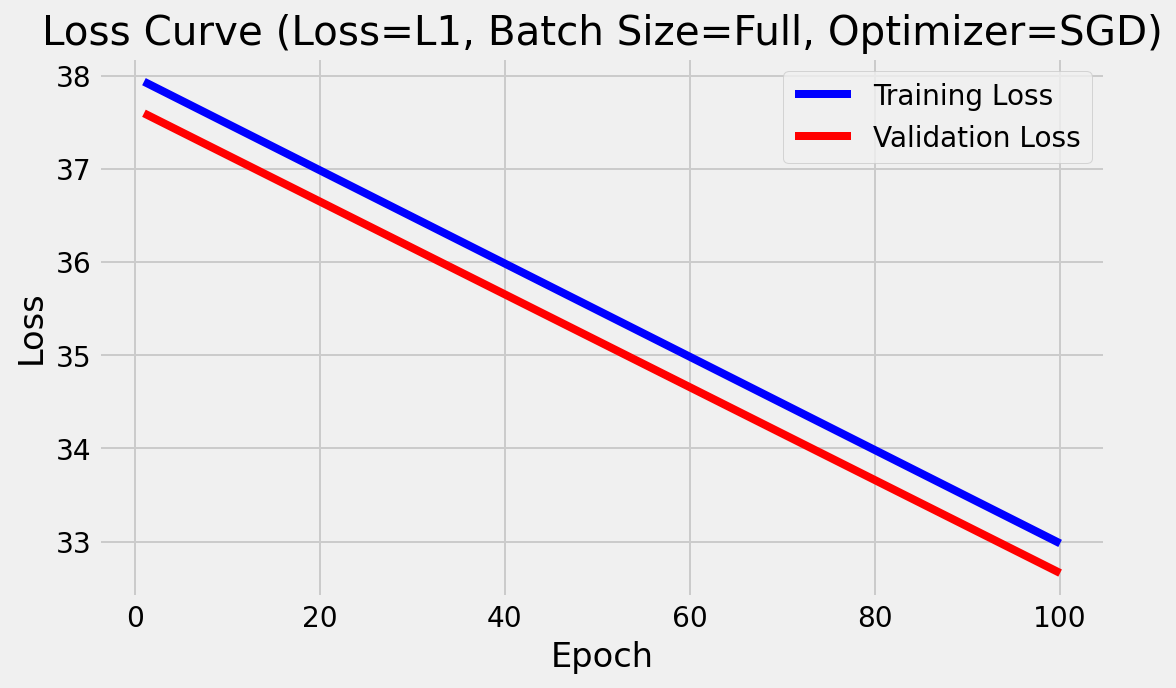
\includegraphics[width=\columnwidth]{figures/c_loss.png}
	\caption{Loss Curve with (\textbf{SGD}, \textbf{L1}, \textbf{full})}
	\label{fig:c loss}
\end{figure}

\LST{part\_c}

In Figure~\ref{fig:c loss} it can be seen that the loss curve takes on a linear shape. This is because the MSE (or L2) loss is computed as square of the difference, giving it that exponential shape. Since L1 loss is computed simple as the difference between $y$ and $\hat{y}$, which is a linear equation the loss curve has a linear shape.